\documentclass[ucs,9pt]{beamer}
% \documentclass[ucs,9pt,handout]{beamer}
\setbeamercovered{transparent}
\newcommand{\semitransp}[2][35]{\color{fg!#1}#2}

\usepackage[utf8x]{inputenc} % Set input encoding to UTF-8.
\usepackage[english]{babel} % Set language.
\usepackage{nicefrac}

% activate KDE theme
\usepackage{KDE/beamerthemeKDE}
\usepackage{tikz}
\usepackage{multicol}
\usepackage{listings}

\title[Device Tailored Wayland Compositors]{Device Tailored Compositors}
\subtitle{with the QtWayland-Compositor Framework}
\author{Andreas Cord-Landwehr}
\date{\textnormal{February 5, 2017\\[\medskipamount] FOSDEM, Brussels}}

\newcommand{\KDEemail}{cordlandwehr@kde.org}
% % % \newcommand{\KDEweb}{https://talks.cord-landwehr.de}
% % % \newcommand{\KDEaffiliation}{KDE Developer}
% % %

\lstset{ %
  language=C,
  backgroundcolor=\color{KDEgray4},
  basicstyle=\footnotesize\ttfamily,
  breakatwhitespace=false,
  breaklines=true,
  captionpos=b,
  commentstyle=\color{KDEgreen},
  escapeinside={\%*}{*)},
  extendedchars=true,
  frame=single,
  keywordstyle=\color{KDEblue},
  language=Prolog,
  numbers=left,
  numbersep=5pt,
  numberstyle=\tiny\color{lightgray},
  rulecolor=\color{lightgray},
  showspaces=false,
  showstringspaces=false,
  showtabs=false,
  stepnumber=1,
  stringstyle=\color{KDEorange},
  tabsize=2,
  title=\lstname,
  morekeywords={Item,import,not,\},\{,Q_SIGNALS,public,Q_OBJECT,virtual,NOTIFY,Q_NULLPTR,Q_DISABLE_COPY,Q_DECL_OVERRIDE},
  deletekeywords={time}
}

%TikZ Definitions
\usetikzlibrary{arrows}
\usetikzlibrary{fit}
\usetikzlibrary{shadows}
\usetikzlibrary{patterns}
\usetikzlibrary{matrix}
\usetikzlibrary{shapes}
\usetikzlibrary{calc}
\usetikzlibrary{decorations.pathmorphing}
\usetikzlibrary{positioning}
\usetikzlibrary{backgrounds}
\usetikzlibrary{decorations}
\usetikzlibrary{decorations.pathreplacing}

\usepackage[variablett]{lmodern}

\newcommand*{\eswap}[3]{#1:[#2\rightarrow#3]}

\begin{document}
\maketitle

\begin{frame}
    {Introduction}
    {About Me \& the Talk}

    \begin{textblock*}{.4\paperwidth}[1,0](\paperwidth,0pt)%
        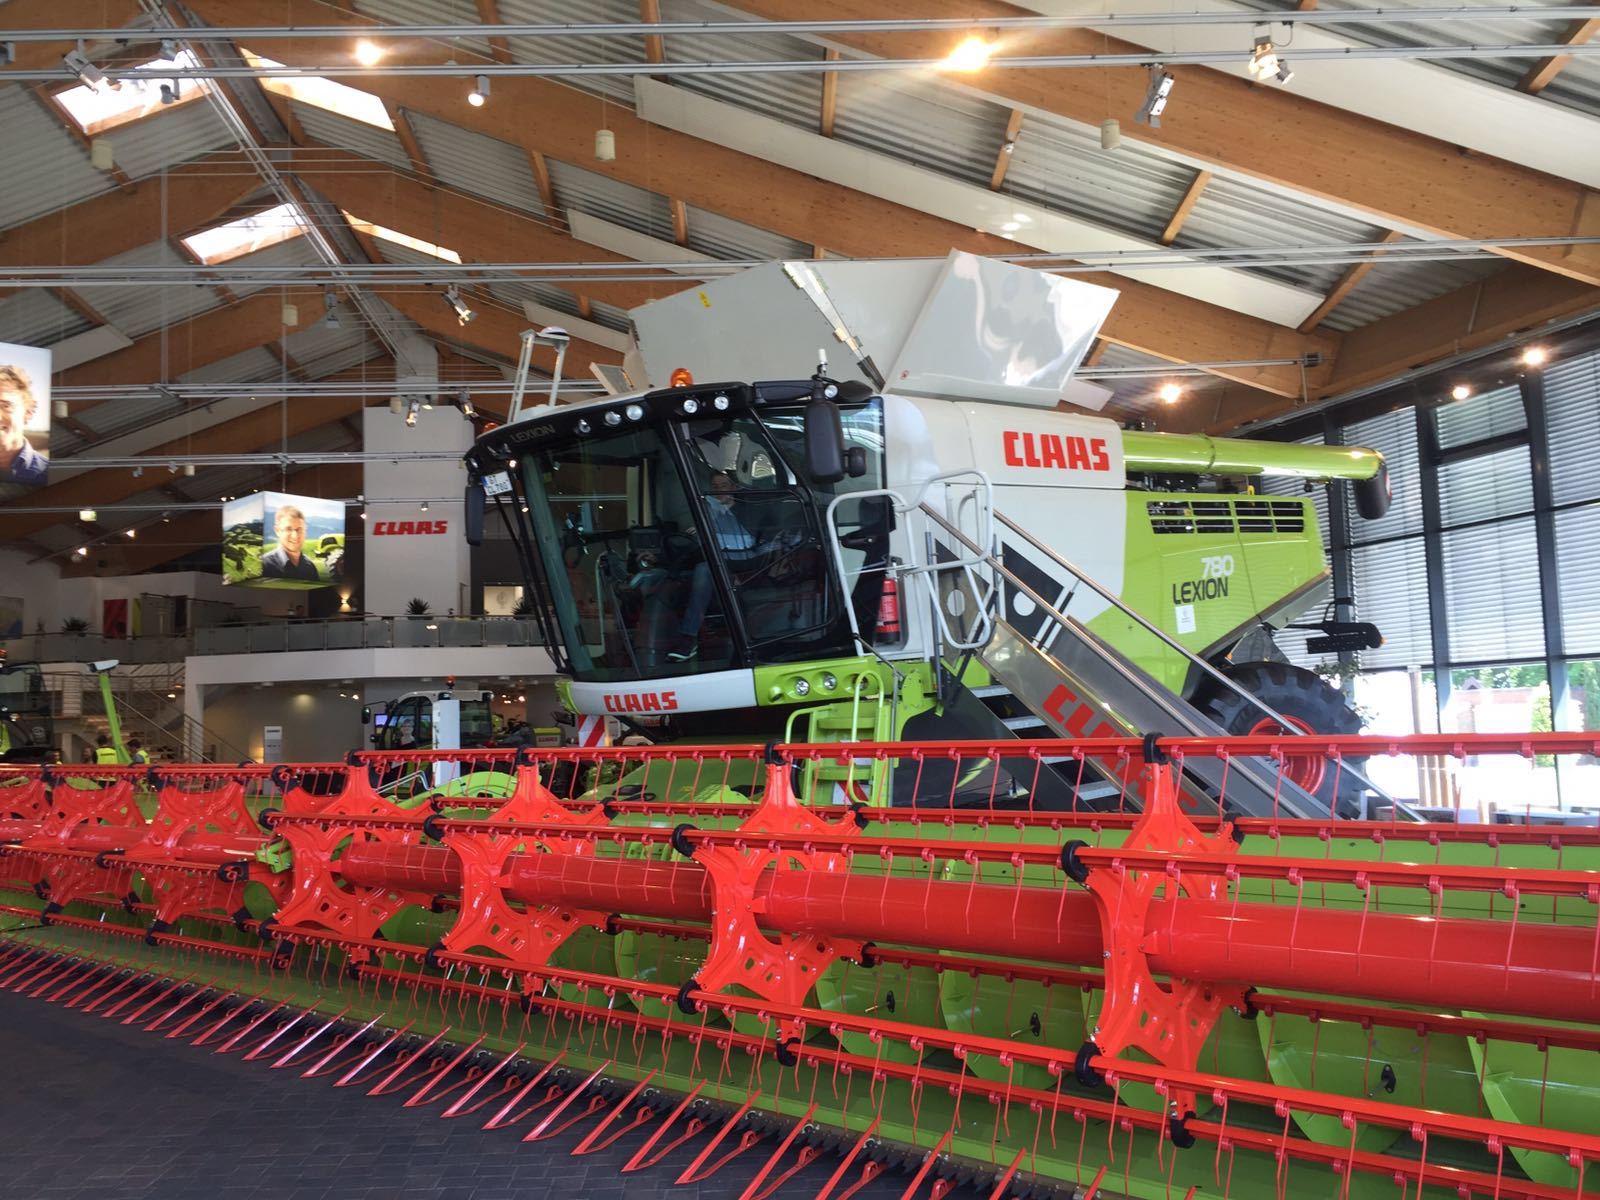
\includegraphics[width=\linewidth]{lexion.jpg}
    \end{textblock*}%

    \textbf{About Me}
    \begin{itemize}
        \item IRC-nick: CoLa
        \item KDE developer since $\approx$ 2010
        \item did PhD in algorithmic game theory\\ at Paderborn University \hspace{2.5cm}$\nearrow$
        \item now working as developer at CLAAS E-Systems in department for displays and operator panels for big agriculture machinery
    \end{itemize}
    \bigskip

    \textbf{This talk is about the QtWayland Compositor Framework:}
    \begin{enumerate}
        \item topic is between my KDE and my professional work
        \item it's a practical introduction how that framework can change how compositors are
        \item the talk shall make you eager to experiment with QtWaylandCompositor
        \item want to convince you that there is a new solution for many embedded device needs
    \end{enumerate}
\end{frame}

\usebackgroundtemplate{%
  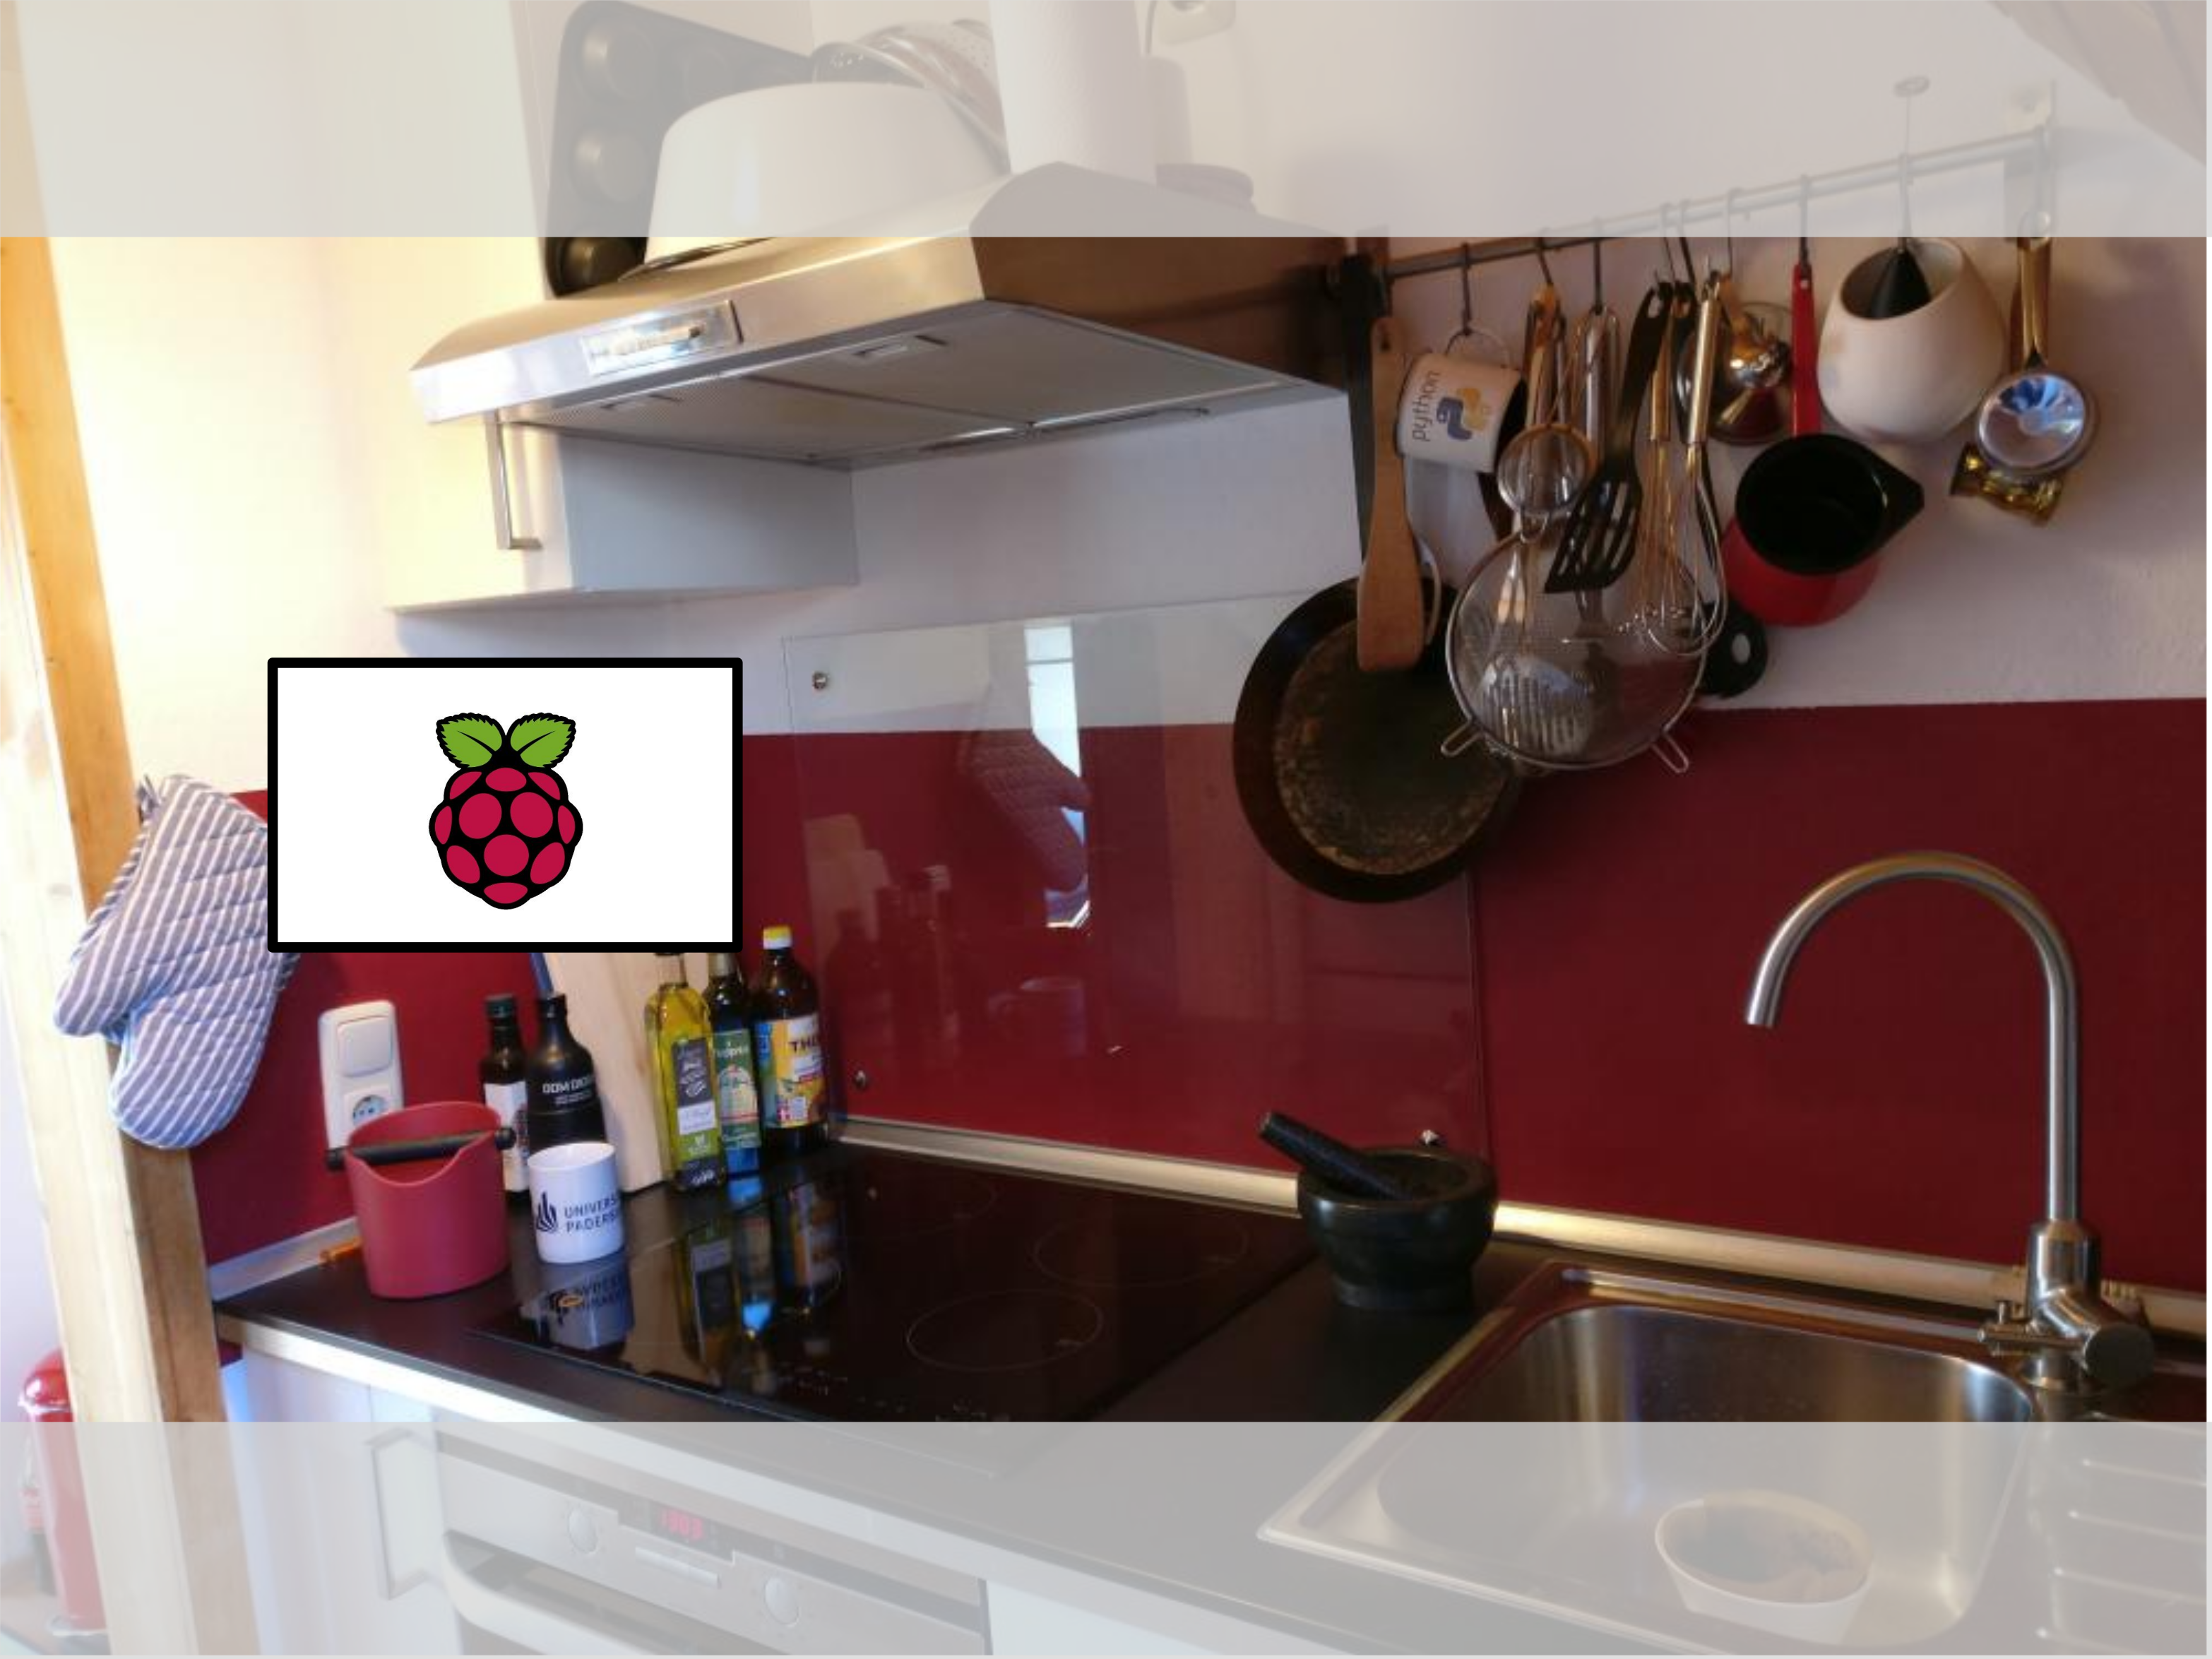
\includegraphics[width=\paperwidth,height=\paperheight]{kitchen-device.png}}

\begin{frame}
    {The Red Thread}
    {Consider an embedded device for my kitchen\dots}
\end{frame}
\usebackgroundtemplate{}

\begin{frame}
    {Requirements \& Consequences}

    \begin{textblock*}{.4\paperwidth}[1,0](\paperwidth,0pt)%
        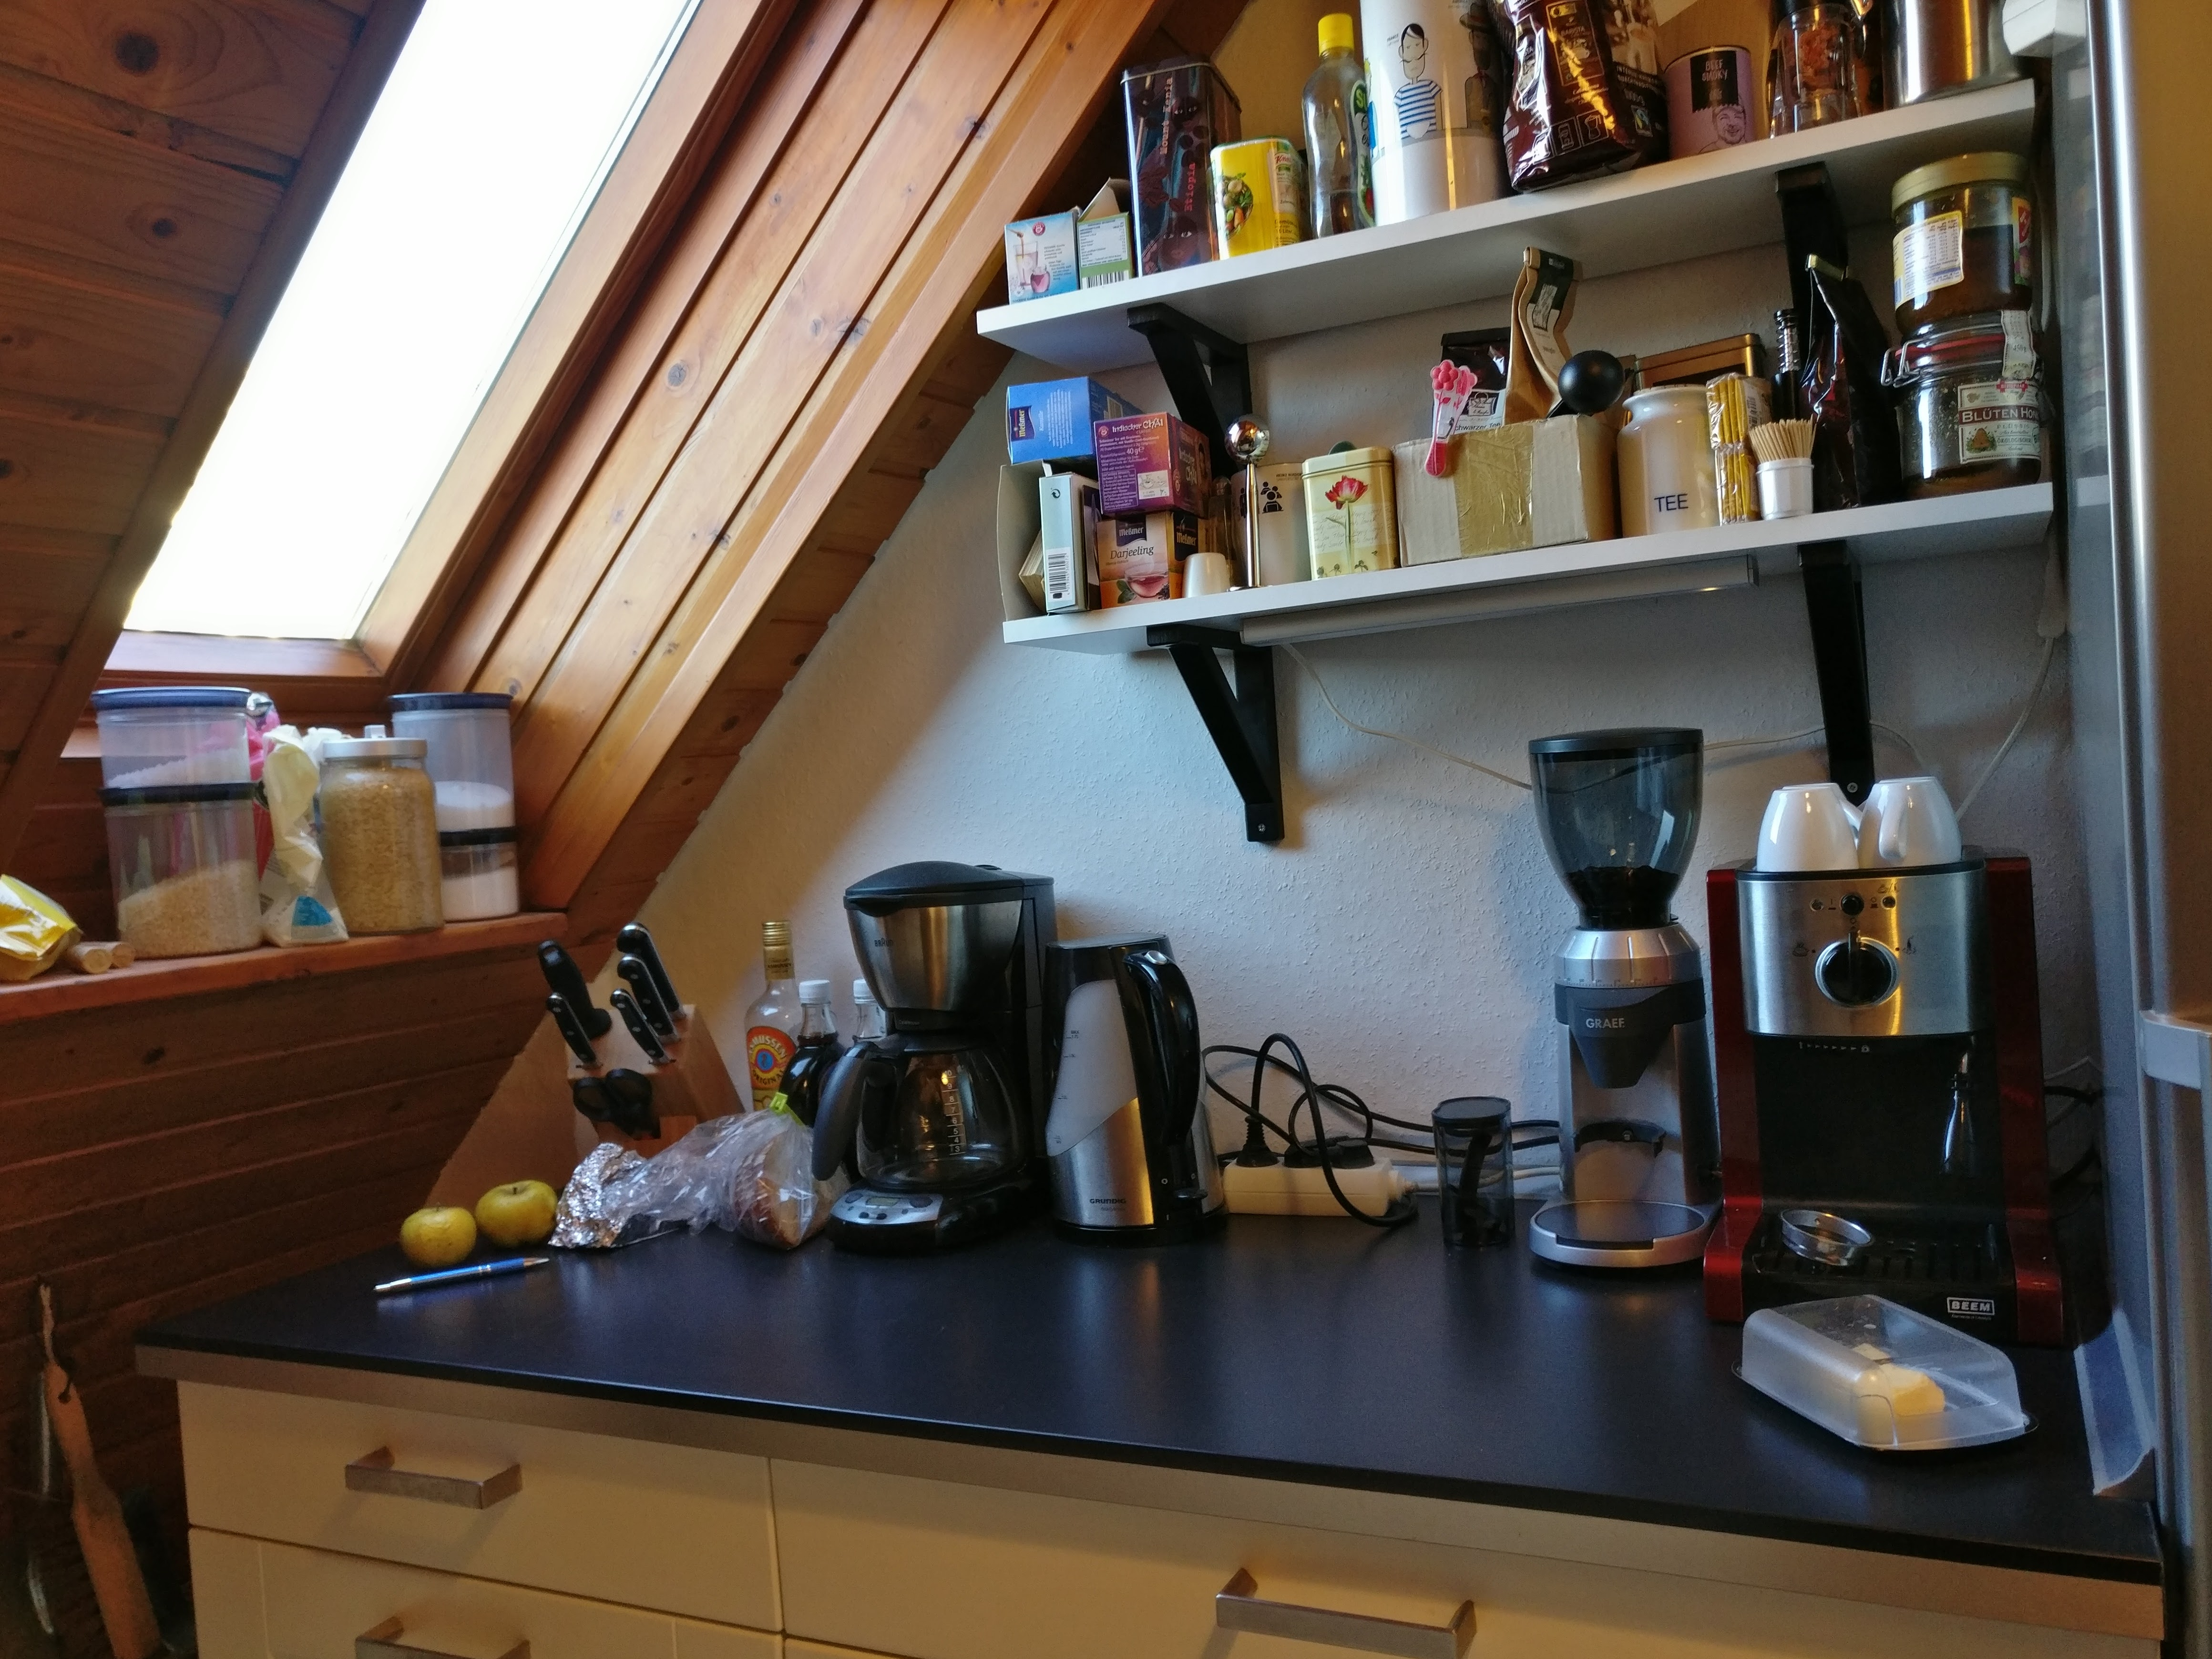
\includegraphics[width=\linewidth]{kitchen-right.jpg}
    \end{textblock*}%

    \begin{itemize}
        \item powerful Linux based device with\\
            3D acceleration (e.g. Raspberry Pi)
        \item multi-application device:
            \begin{itemize}
                \item cooking eggs timer
                \item tea timer
                \item a game
            \end{itemize}
        \item animations and touch handling for changing applications
        \item seemless UI between the application windows
        \item [$\rightarrow$] we need a Wayland compositor
    \end{itemize}
    \bigskip

    \emph{Yes, the above can be reached in a much simpler way, but exchanging the trivial apps with an internet radio, a navigation system etc.\ and you get what modern cars put onto their devices.}
\end{frame}

\begin{frame}
    {Interaction Concept}
    {Let's keep it simple for the talk}

    \alert{add it once demo is finished :)}

\end{frame}


\begin{frame}
    {A System Architecture for my Kitchen Control}

    \begin{textblock*}{.4\paperwidth}[1,0](.95\paperwidth,.125\paperheight)%
        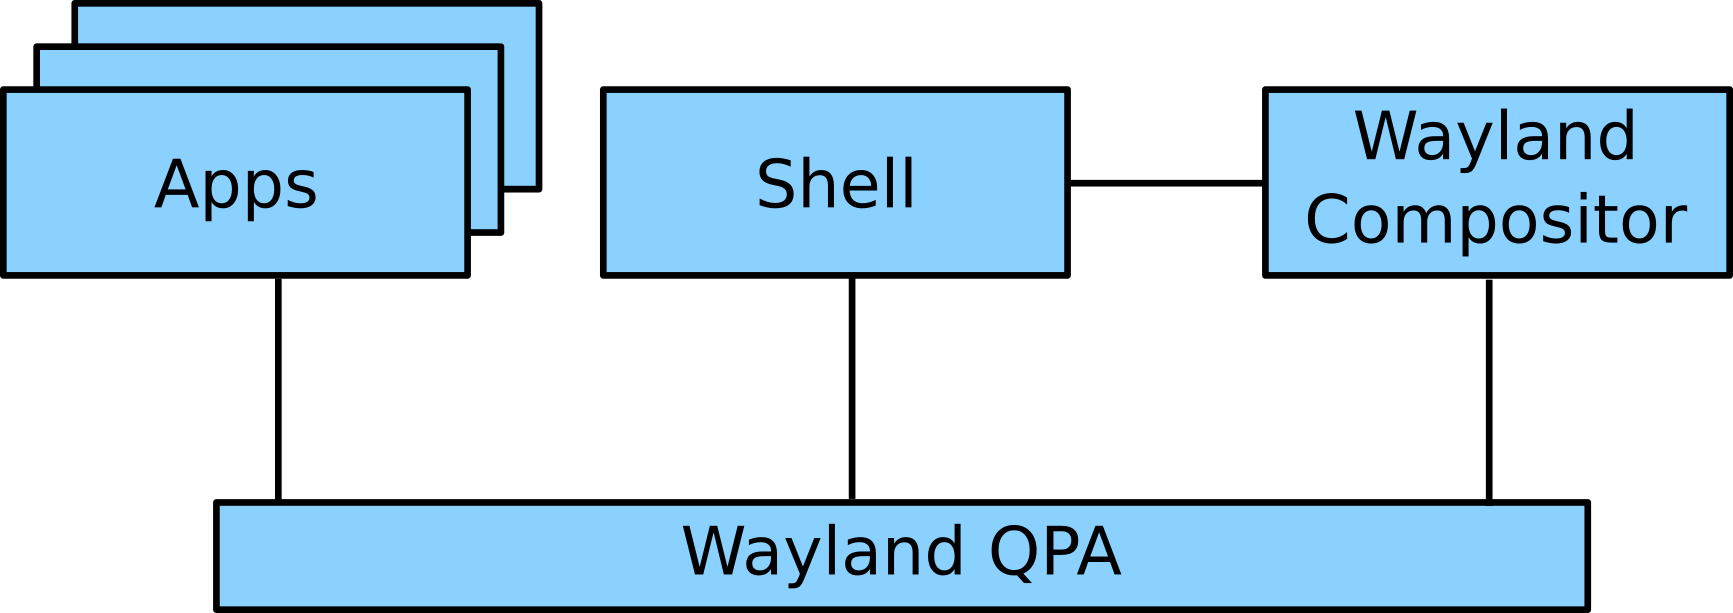
\includegraphics[width=\linewidth]{architecture.png}
    \end{textblock*}%

    \begin{description}
        \item [apps] Qt application run on Wayland\\
            QPA ({\tt -platform wayland}) $\rightarrow$ Qt handles everything for us
        \item [compositor] application acting as Wayland Server
        \item [shell] application that handles the more complex compositing logic and provides
            standard screens (loading, dialogs\dots)
    \end{description}
    \bigskip

    Note: separating logic between the Shell and the Compositor is mostly a matter of taste
\end{frame}

\begin{frame}
    {Wayland Compositer by QtWayland}
    {What it does and the new API}

    \textbf{The New QtWayland Compositor API}
    \begin{itemize}
        \item possible to write a compositor in only QML
        \item Wayland protocol extension support
        \item multi-screen support
        \item provides XDG-Shell and IVI-Shell interfaces
        \item History:
            \begin{itemize}
                \item since many years, there was an internal (cumbersome to use) API
                \item Compositor API rewritten for Qt 5.7 (tech preview)
                \item Stable API since Qt 5.8 \alert{check if release happened until today}
            \end{itemize}
    \end{itemize}
    \medskip

    \textbf{Alternatives:} What about using the IVI-Shell extension?
    \begin{itemize}
        \item protocol only suited for very static settings
        \item Qt event loop handling not always well handled by off-the-shelf compositors
    \end{itemize}
\end{frame}

\begin{frame}
    {A Wayland Compositor on One Slide}
    \alert{copy from demo}
\end{frame}

\begin{frame}
    {Protocol Extension for Alarm Notifications}
    \alert{copy from demo}
\end{frame}

\begin{frame}
    {Demo}
\end{frame}

\begin{frame}
    {References}

    \begin{itemize}
        \item Johan's talk at QtCon 2016: structured introduction into the framework
        \item online help
        \item examples
        \item \dots
    \end{itemize}
\end{frame}

\KDElastframe

\end{document}
